% ============================================================================
% INTRODUCTION GÉNÉRALE — VERSION SCRUM
% ============================================================================

\section{Contexte et Motivation}

Le tourisme représente un pilier essentiel de l'économie tunisienne, contribuant à hauteur de 
14\% du PIB national et générant plus de 2 millions d'emplois directs et indirects. L'île de 
Djerba, avec ses plages paradisiaques, son patrimoine culturel unique et son climat méditerranéen, 
attire ежегодно plus de 3 millions de visiteurs internationaux. Cependant, malgré ce potentiel 
exceptionnel, les touristes font face à des défis majeurs lors de la planification de leur séjour~: 
la dispersion des informations, la barrière linguistique (français, anglais, arabe), et l'absence 
de recommandations véritablement personnalisées adaptées à leur profil et contexte de voyage.

Les plateformes de voyage existantes se divisent en deux catégories principales. D'une part, les 
moteurs de recherche génériques (Booking.com, TripAdvisor, Expedia) offrent un catalogue exhaustif 
mais imposent une navigation fastidieuse à travers des filtres multiples, sans compréhension 
sémantique des besoins implicites de l'utilisateur. D'autre part, les agents conversationnels 
récents basés sur les grands modèles de langage (LLM) produisent des réponses fluides mais 
souffrent d'hallucinations factuelles critiques~: ils inventent des prix, des adresses inexistantes 
ou des horaires erronés, détruisant ainsi la confiance utilisateur dès la première interaction.

Le projet Guidni émerge de ce constat avec une ambition double~: concevoir un planificateur de 
voyage conversationnel multilingue qui combine l'intelligence naturelle des LLM avec l'ancrage 
factuel d'une base de données locale vérifiée, et développer un moteur de recommandation adaptatif 
qui apprend en temps réel des préférences contextuelles des utilisateurs pour affiner ses 
suggestions au fil des interactions.

\section{Problématique}

La question centrale qui guide ce travail de fin d'études est la suivante~:

\begin{quote}
\textit{« Comment concevoir et implémenter une plateforme intelligente de planification et de 
recommandation touristique pour Djerba qui combine un agent conversationnel multilingue basé sur 
les LLM avec un moteur de recommandation adaptatif par apprentissage en ligne, tout en garantissant 
la fiabilité des informations fournies et l'adaptation aux préférences contextuelles des 
utilisateurs ? »}
\end{quote}

Cette problématique soulève plusieurs défis techniques majeurs. Premièrement, l'intégration d'un 
LLM dans un système de production nécessite de résoudre le problème des hallucinations~: comment 
permettre au modèle de raisonner et de générer des plans cohérents tout en s'assurant que toutes 
les informations factuelles (prix, adresses, horaires) proviennent de sources vérifiées ? 
Deuxièmement, la personnalisation en temps réel exige un algorithme capable d'apprendre 
continuellement à partir de signaux comportementaux faibles (clics, temps de consultation, 
ajouts aux favoris) sans nécessiter de grandes quantités de données historiques. Troisièmement, 
le support multilingue (français, anglais, arabe) impose une architecture capable de détecter 
automatiquement la langue de l'utilisateur et de maintenir la cohérence sémantique across les 
trois langues dans la récupération d'informations et la génération de réponses.

\section{Objectifs du Projet}

Les objectifs de ce projet se déclinent en quatre axes principaux~:

\textbf{Objectif 1~: Agent Planificateur Conversationnel.} Développer un agent basé sur LangGraph 
avec une machine à états explicite orchestrant le cycle de raisonnement ReAct (Reason + Act) en 
quatre nœuds~: THINK (analyse de la situation), EXECUTE\_TOOL (appel des 18 outils spécialisés), 
VALIDATE (vérification de la cohérence structurelle du plan), et RESPOND (formulation de la 
réponse finale). L'agent doit supporter le multilinguisme complet et la gestion de conversations 
longues via un système de mémoire avec résumé automatique.

\textbf{Objectif 2~: Pipeline RAG Multilingue.} Implémenter un système de génération augmentée 
par récupération (RAG) indexant six types d'entités touristiques (activités, hébergements, 
restaurants, attractions, locations, transferts) avec des embeddings denses BAAI/bge-m3 
supportant le français, l'anglais et l'arabe dans un espace sémantique unifié. Le pipeline doit 
inclure une réindexation incrémentale automatique lors des mises à jour de la base de données.

\textbf{Objectif 3~: Moteur de Recommandation LinUCB.} Concevoir un bandit multi-bras contextuel 
utilisant un vecteur de caractéristiques de Kronecker de 360 dimensions ($\phi = x_{user}(9) 
\otimes x_{tags}(40)$) capturant les interactions entre signaux utilisateur (heure, mois, 
comportement, historique) et tags des annonces. Le moteur doit inclure un pipeline de classement 
post-LinUCB en 10 étapes et un mécanisme de récompenses delta par session empêchant l'inflation 
des signaux.

\textbf{Objectif 4~: Intégration Système et Déploiement.} Assurer l'intégration transparente des 
deux sous-systèmes avec la base de données PostgreSQL existante de la plateforme Guidni, sans 
conflit avec le frontend Next.js/Prisma. Déployer le système sur un serveur unique avec des 
endpoints REST documentés, un tableau de bord administrateur pour la reconstruction manuelle de 
l'index RAG, et un monitoring des performances en temps réel.

\section{Structure du Rapport}

Ce rapport est organisé en huit chapitres suivant la méthodologie Scrum adoptée pour le 
développement du projet~:

\textbf{Chapitre 1 — Introduction Générale.} Ce chapitre présente le contexte, la problématique, 
les objectifs et la méthodologie Scrum choisie pour mener à bien ce projet de fin d'études.

\textbf{Chapitre 2 — Contexte Général et Étude Préliminaire.} Ce chapitre décrit l'organisme 
d'accueil (ISITCOM), présente une étude approfondie de l'existant dans les domaines des chatbots 
et systèmes de recommandation, établit le cahier des charges fonctionnel et technique, et détaille 
la méthodologie Scrum avec ses rôles, artefacts et cérémonies.

\textbf{Chapitre 3 — Lancement de Projet.} Ce chapitre couvre l'analyse des besoins, l'architecture 
globale du système, la construction du Product Backlog avec priorisation MoSCoW, la planification 
des quatre sprints, et la définition des critères de qualité (Definition of Done).

\textbf{Chapitre 4 — Sprint 1 : Conception et Implémentation de l'Agent Planificateur.} Ce 
chapitre présente les livrables du premier sprint~: la machine à états LangGraph, les 18 outils 
appelables, le pipeline RAG multilingue, et le système de mémoire conversationnelle.

\textbf{Chapitre 5 — Sprint 2 : Implémentation du Moteur de Recommandation Hybrid LinUCB.} Ce 
chapitre détaille le deuxième sprint consacré au moteur de recommandation~: ingénierie des 
caractéristiques avec vecteur de Kronecker, algorithme LinUCB, pipeline de classement en 10 
étapes, et tracker JavaScript pour la collecte des événements.

\textbf{Chapitre 6 — Sprint 3 : Tests et Évaluation.} Ce chapitre expose la stratégie de tests 
(unitaires, intégration, évaluation empirique), les scénarios de test pour l'agent planificateur 
et le moteur LinUCB, et les résultats obtenus en termes de précision, latence et récompense 
cumulée.

\textbf{Chapitre 7 — Sprint 4 : Intégration et Déploiement.} Ce chapitre final décrit 
l'intégration des deux sous-systèmes, le déploiement en environnement de production, les endpoints 
de santé et de monitoring, et la démonstration finale de la plateforme complète.

\textbf{Conclusion Générale et Perspectives.} La conclusion synthétise les contributions majeures 
du projet et propose cinq pistes de travaux futurs~: fine-tuning d'un LLM local, remplacement du 
LinUCB linéaire par un bandit neuronal, infrastructure d'expérimentation A/B, extension 
multi-régions, et interface vocale multimodale.

% ────────────────────────────────────────────────────────────────
\section{Méthodologie Scrum}
% ────────────────────────────────────────────────────────────────

\subsection{Pourquoi Scrum ?}

Le choix de la méthodologie Scrum pour ce projet de fin d'études s'impose pour plusieurs raisons 
fondamentales liées à la nature même du domaine de l'intelligence artificielle et aux contraintes 
académiques du PFE.

\textbf{Incertitude inhérente à l'IA.} Les projets d'IA comportent une incertitude technique 
importante~: les performances réelles des modèles LLM, la qualité des embeddings multilingues, 
et la convergence de l'algorithme LinUCB ne peuvent être prédites avec certitude avant 
l'expérimentation. Scrum permet d'embrasser cette incertitude en livrant des incréments 
fonctionnels à chaque sprint, permettant ainsi d'ajuster la trajectoire du projet en fonction 
des résultats observés plutôt que de suivre un plan rigide établi a priori.

\textbf{Livraison itérative de valeur.} La décomposition en quatre sprints de trois semaines 
chacun permet de livrer progressivement des fonctionnalités opérationnelles~: l'agent 
planificateur (Sprint 1), le moteur de recommandation (Sprint 2), les tests complets (Sprint 3), 
et l'intégration-déploiement (Sprint 4). Chaque livraison peut être démontrée au superviseur et 
potentiellement utilisée par des testeurs précoces, générant des retours exploitables pour les 
sprints suivants.

\textbf{Adéquation avec le calendrier académique.} Le format itératif de Scrum s'aligne 
naturellement avec le rythme universitaire~: chaque sprint correspond approximativement à une 
période de vacances intermédiaire, permettant des points d'étape formels avec l'encadrant. La 
documentation requise par Scrum (Product Backlog, Sprint Backlog, Definition of Done) constitue 
également une ossature idéale pour la rédaction du rapport de PFE.

\textbf{Flexibilité face aux imprévus.} Un projet de fin d'études comporte inévitablement des 
aléas~: difficultés techniques imprévues, évolution des exigences, contraintes de temps. Scrum 
offre un cadre structuré pour gérer ces imprévus~: si une user story ne peut être terminée dans 
un sprint, elle est replanifiée au sprint suivant sans compromettre l'ensemble du projet.

\begin{figure}[H]
    \centering
    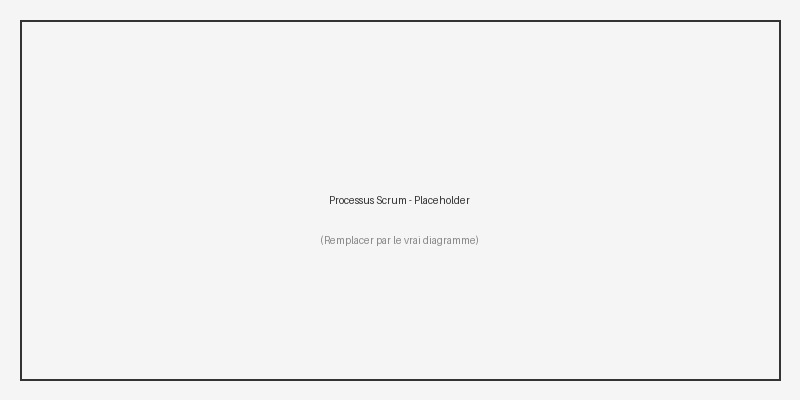
\includegraphics[width=0.85\textwidth]{diagrams/fig_01_scrum_process.png}
    \caption{Cycle du processus Scrum adapté au projet Guidni}
    \label{fig:scrum_process}
\end{figure}

La figure~\ref{fig:scrum_process} illustre le cycle Scrum adopté~: chaque sprint commence par 
une phase de \textbf{Sprint Planning} où les user stories sont sélectionnées depuis le Product 
Backlog et décomposées en tâches techniques. Le développement suit ensuite avec des \textbf{Daily 
Scrums} quotidiens (auto-évaluation individuelle) pour synchroniser l'avancement. Le sprint se 
termine par une \textbf{Sprint Review} avec le superviseur pour démontrer les fonctionnalités 
implémentées, suivie d'une \textbf{Sprint Retrospective} pour identifier les améliorations de 
processus applicables au sprint suivant.

\subsection{Rôles Scrum}

Le tableau~\ref{tab:scrum_roles} définit les rôles Scrum tels qu'attribués dans le cadre de ce 
projet de fin d'études.

\begin{table}[H]
    \centering
    \caption{Rôles Scrum dans le projet Guidni}
    \label{tab:scrum_roles}
    \small
    \begin{tabular}{p{3cm} p{4cm} p{6cm}}
        \toprule
        \textbf{Rôle} & \textbf{Titulaire} & \textbf{Responsabilités} \\
        \midrule
        Product Owner (PO) & Superviseur académique & Définir la vision produit, prioriser le 
        Product Backlog, valider les livrables en Sprint Review, arbitrer les compromis 
        fonctionnels. \\
        \midrule
        Scrum Master (SM) & Étudiant (Ahmed Addali) & Faciliter les cérémonies Scrum, lever les 
        obstacles, garantir le respect du cadre Scrum, assurer la vélocité de l'équipe. \\
        \midrule
        Équipe de Développement & Étudiant (Ahmed Addali) & Concevoir, implémenter et tester les 
        fonctionnalités, estimer les charges, s'engager sur le Sprint Backlog, produire des 
        incréments potentiellement livrables. \\
        \bottomrule
    \end{tabular}
\end{table}

Dans le contexte spécifique d'un PFE individuel, l'étudiant cumule les rôles de Scrum Master et 
de développeur unique, tandis que le superviseur académique assume le rôle de Product Owner. Cette 
configuration simplifiée conserve néanmoins l'essentiel des bénéfices de Scrum~: la séparation 
des responsabilités entre la définition du \textit{quoi} (PO) et la réalisation du \textit{comment} 
(équipe), et l'amélioration continue via les rétrospectives.

% ────────────────────────────────────────────────────────────────
\section{Planification des Sprints}
% ────────────────────────────────────────────────────────────────

Le projet Guidni est découpé en quatre sprints de trois semaines chacun, couvrant la période 
totale de douze semaines allouée au développement. La figure~\ref{fig:gantt_sprints} présente 
le diagramme de Gantt global du projet.

\begin{figure}[H]
    \centering
    \includegraphics[width=\textwidth]{diagrams/fig_01_gantt_sprints.png}
    \caption{Diagramme de Gantt des quatre sprints du projet Guidni}
    \label{fig:gantt_sprints}
\end{figure}

Le tableau~\ref{tab:sprint_planning} résume les objectifs, périodes et livrables clés de chaque 
sprint.

\begin{table}[H]
    \centering
    \caption{Planification des sprints}
    \label{tab:sprint_planning}
    \small
    \begin{tabular}{p{2cm} p{4.5cm} p{3cm} p{4cm}}
        \toprule
        \textbf{Sprint} & \textbf{Objectif Principal} & \textbf{Période} & \textbf{Livrables} \\
        \midrule
        Sprint 1 & Agent planificateur IA avec LangGraph, RAG et mémoire & Semaines 1--3 & Graphe 
        LangGraph 4 nœuds, 18 outils, pipeline RAG bge-m3, mémoire conversationnelle, endpoint 
        /chat \\
        \midrule
        Sprint 2 & Moteur de recommandation Hybrid LinUCB & Semaines 4--6 & Ingénierie des 
        caractéristiques (360D), algorithme LinUCB, ranker 10 étapes, tracker JS, jobs nocturnes \\
        \midrule
        Sprint 3 & Tests complets et évaluation empirique & Semaines 7--9 & Tests unitaires 
        (context, linucb, ranker), tests d'intégration (/chat, /plan, /events), évaluation 
        manuelle, métriques de performance \\
        \midrule
        Sprint 4 & Intégration, déploiement et démo finale & Semaines 10--12 & Intégration des 
        deux sous-systèmes, endpoints de santé, dashboard admin, documentation API, démonstration 
        complète \\
        \bottomrule
    \end{tabular}
\end{table}

Chaque sprint suit le même déroulement type~:
\begin{itemize}
    \item \textbf{Jour 1~:} Sprint Planning (2--4 heures) -- Sélection des user stories, 
          estimation T-Shirt (XS à XL), création du Sprint Backlog.
    \item \textbf{Jours 2--18~:} Développement avec Daily Scrum quotidien (15 minutes 
          d'auto-évaluation) et avancement selon les tâches définies.
    \item \textbf{Jour 19~:} Sprint Review (1--2 heures avec le superviseur) -- Démonstration 
          des fonctionnalités implémentées, validation des critères d'acceptation.
    \item \textbf{Jour 20~:} Sprint Retrospective (1 heure) -- Analyse des points forts, 
          faiblesses et actions d'amélioration pour le sprint suivant.
\end{itemize}

La vélocité cible est de 8 à 10 points de story par sprint, basée sur une échelle de complexité 
relative où une story XS vaut 1 point, S vaut 2 points, M vaut 4 points, L vaut 8 points et XL 
vaut 13 points. Cette granularité permet un suivi précis de la charge réelle versus la charge 
estimée.

\section{Conclusion de l'Introduction}

Ce chapitre introductif a posé les fondations du projet Guidni en présentant le contexte 
touristique de Djerba, la problématique centrale combinant fiabilité des LLM et personnalisation 
en temps réel, les quatre objectifs techniques majeurs, et la méthodologie Scrum structurée en 
quatre sprints thématiques. Les chapitres suivants détailleront successivement le cadre général 
et l'étude préliminaire (Chapitre 2), le lancement de projet avec l'architecture et le Product 
Backlog (Chapitre 3), puis les réalisations concrètes de chaque sprint (Chapitres 4 à 7).
